\documentclass[10pt,a4paper,landscape]{article}
\usepackage[utf8]{inputenc}
\usepackage[english]{babel}
\usepackage{graphicx}
\usepackage{pgf-umlcd}
\usepackage{textcomp}


\begin{document}
\renewcommand{\umlfillcolor}{white}
\renewcommand{\umldrawcolor}{black}
\renewcommand{\umltextcolor}{black}
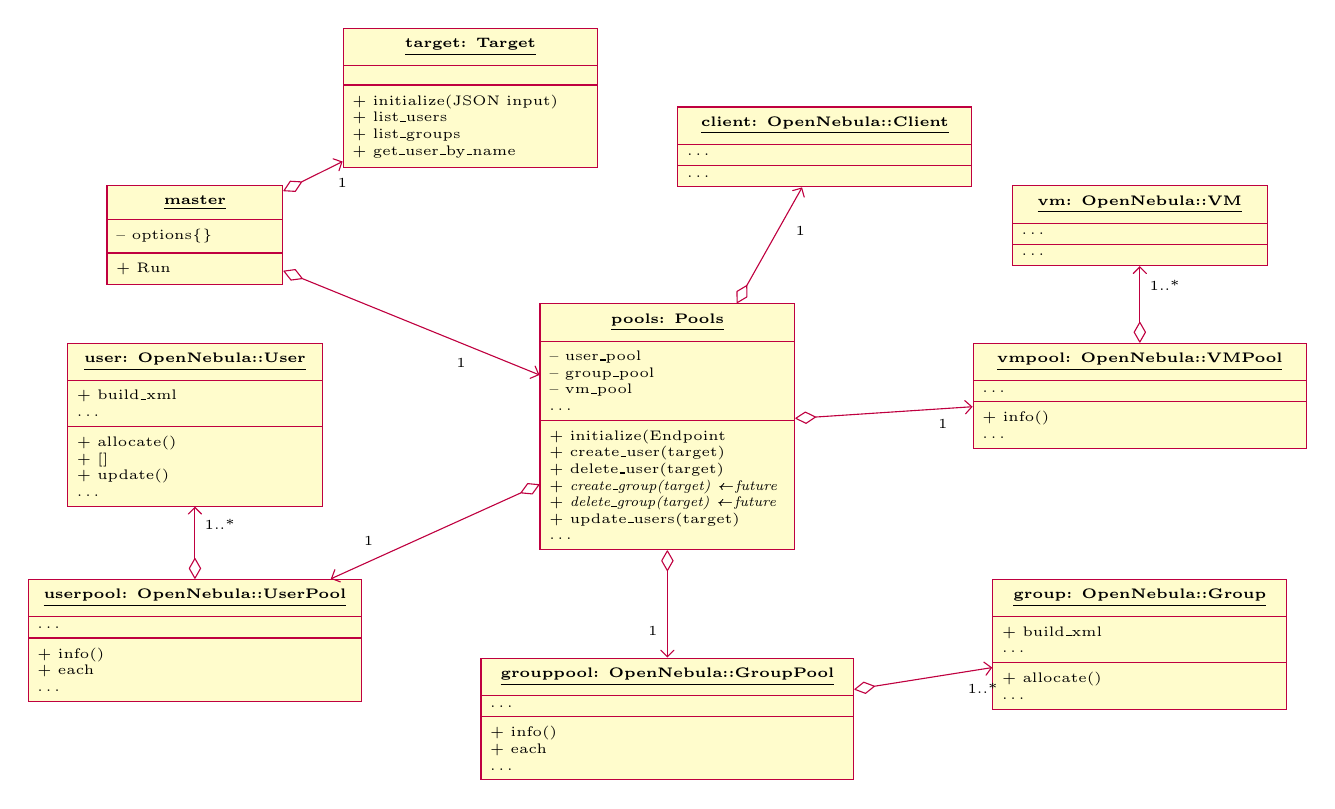
\begin{tikzpicture}
  \tikzstyle{every node}=[font=\tiny]

  \begin{object}[text width=2cm]{master}{0,6}
	\attribute{-- options\{\}}
	\operation{+ Run}
  \end{object}


  \begin{object}[text width=3cm]{target}{3.5,8}
	\instanceOf{Target}
	\operation{+ initialize(JSON input)}
	\operation{+ list\_users}
	\operation{+ list\_groups}
	\operation{+ get\_user\_by\_name}
  \end{object}


  \begin{object}[text width=3cm]{pools}{6,4.5}
	\instanceOf{Pools}
	\attribute{-- user\_pool}
	\attribute{-- group\_pool}
	\attribute{-- vm\_pool}
	\attribute{\dots}
	\operation{+ initialize(Endpoint}
	\operation{+ create\_user(target)}
	\operation{+ delete\_user(target)}
	\operation{+ \textit{create\_group(target) \textleftarrow future}}
	\operation{+ \textit{delete\_group(target) \textleftarrow future}}
	\operation{+ update\_users(target)}
	\operation{\dots}
  \end{object}

  
  \begin{object}[text width=3cm]{user}{0,4}
	\instanceOf{OpenNebula::User}
	\attribute{+ build\_xml}
	\attribute{\dots}
	\operation{+ allocate()}
	\operation{+ []}
	\operation{+ update()}
	\operation{\dots}
  \end{object}


  \begin{object}[text width=4cm]{userpool}{0,1}
	\instanceOf{OpenNebula::UserPool}
	\attribute{\dots}
	\operation{+ info()}
	\operation{+ each}
	\operation{\dots}
  \end{object}


  \begin{object}[text width=4.5cm]{grouppool}{6,0}
	\instanceOf{OpenNebula::GroupPool}
	\attribute{\dots}
	\operation{+ info()}
	\operation{+ each}
	\operation{\dots}
  \end{object}


  \begin{object}[text width=3.5cm]{group}{12,1}
	\instanceOf{OpenNebula::Group}
	\attribute{+ build\_xml}
	\attribute{\dots}
	\operation{+ allocate()}
	\operation{\dots}
  \end{object}


  \begin{object}[text width=4cm]{vmpool}{12,4}
	\instanceOf{OpenNebula::VMPool}
	\attribute{\dots}
	\operation{+ info()}
	\operation{\dots}
  \end{object}


  \begin{object}[text width=3cm]{vm}{12,6}
	\instanceOf{OpenNebula::VM}
	\attribute{\dots}
	\operation{\dots}
  \end{object}


  \begin{object}[text width=3.5cm]{client}{8,7}
	\instanceOf{OpenNebula::Client}
	\attribute{\dots}
	\operation{\dots}
  \end{object}


%  \association{SSHandHTTPS}{id}{}{ApplySSHandHTTPS}{}{target}
   \aggregation{userpool}{}{1..*}{user}
   \aggregation{grouppool}{}{1..*}{group}
   \aggregation{vmpool}{}{1..*}{vm}
   \aggregation{pools}{}{1}{userpool}
   \aggregation{pools}{}{1}{grouppool}
   \aggregation{pools}{}{1}{vmpool}
   \aggregation{pools}{}{1}{client}
   \aggregation{master}{}{1}{target}
   \aggregation{master}{}{1}{pools}


\end{tikzpicture}

\end{document}
